\documentclass[11pt]{beamer}
\usepackage[utf8]{inputenc}
\usepackage[T1]{fontenc}
\usepackage{lmodern}
\usepackage{amsfonts}
\usepackage{amsmath}
\usepackage{amssymb}
\usepackage{ragged2e}
\usepackage{graphicx}
\usepackage{subcaption}
\usepackage{natbib}
\usetheme{Madrid}
\usecolortheme{orchid}
\setbeamertemplate{navigation symbols}{}
\setbeamertemplate{footline}[frame number]{}
	\author{Ruben \textsc{Espeleta Bolivar} \\
	\and {Advisor: Dr. Cruz \textsc{García Molina}}}
\title[Numerical experiments]{Numerical experiments in idealized glacier topographies}
\date[KPT 2004]{Presented in the partial fulfillment of the requirements for the degree of \\
Master applied mechanics}

\subtitle{Case study of the impact of the mesh resolution on the prediction of the grounding line position}
\logo{
\includegraphics[scale=0.15]{../fig/logo_IGE.png}}
\institute[IGE]{
	\inst{1}
	Institut des geosciences de l'environnement
}

%\setbeamercovered{transparent}
%\setbeamertemplate{navigation symbols}{}
%\AtBeginSection[]{
%	\begin{frame}<beamer>{Contenido}
%		\tableofcontents[currentsection]
%	\end{frame}
%}
\begin{document}

	\begin{frame}
		\maketitle
	\end{frame}
	
	\begin{frame}{Content}
		\tableofcontents[hideallsubsections]
	\end{frame}
	
	\section{Introduction}
	\subsection{Definition}
		\begin{frame}{What is a glacier?}
		\justifying
		Glaciers can be defined as a mass of ice that accumulates from snow and flows downwards from a few hundreds of meters per year and up to 15 km per year.\pause
		\begin{figure}
		\centering
		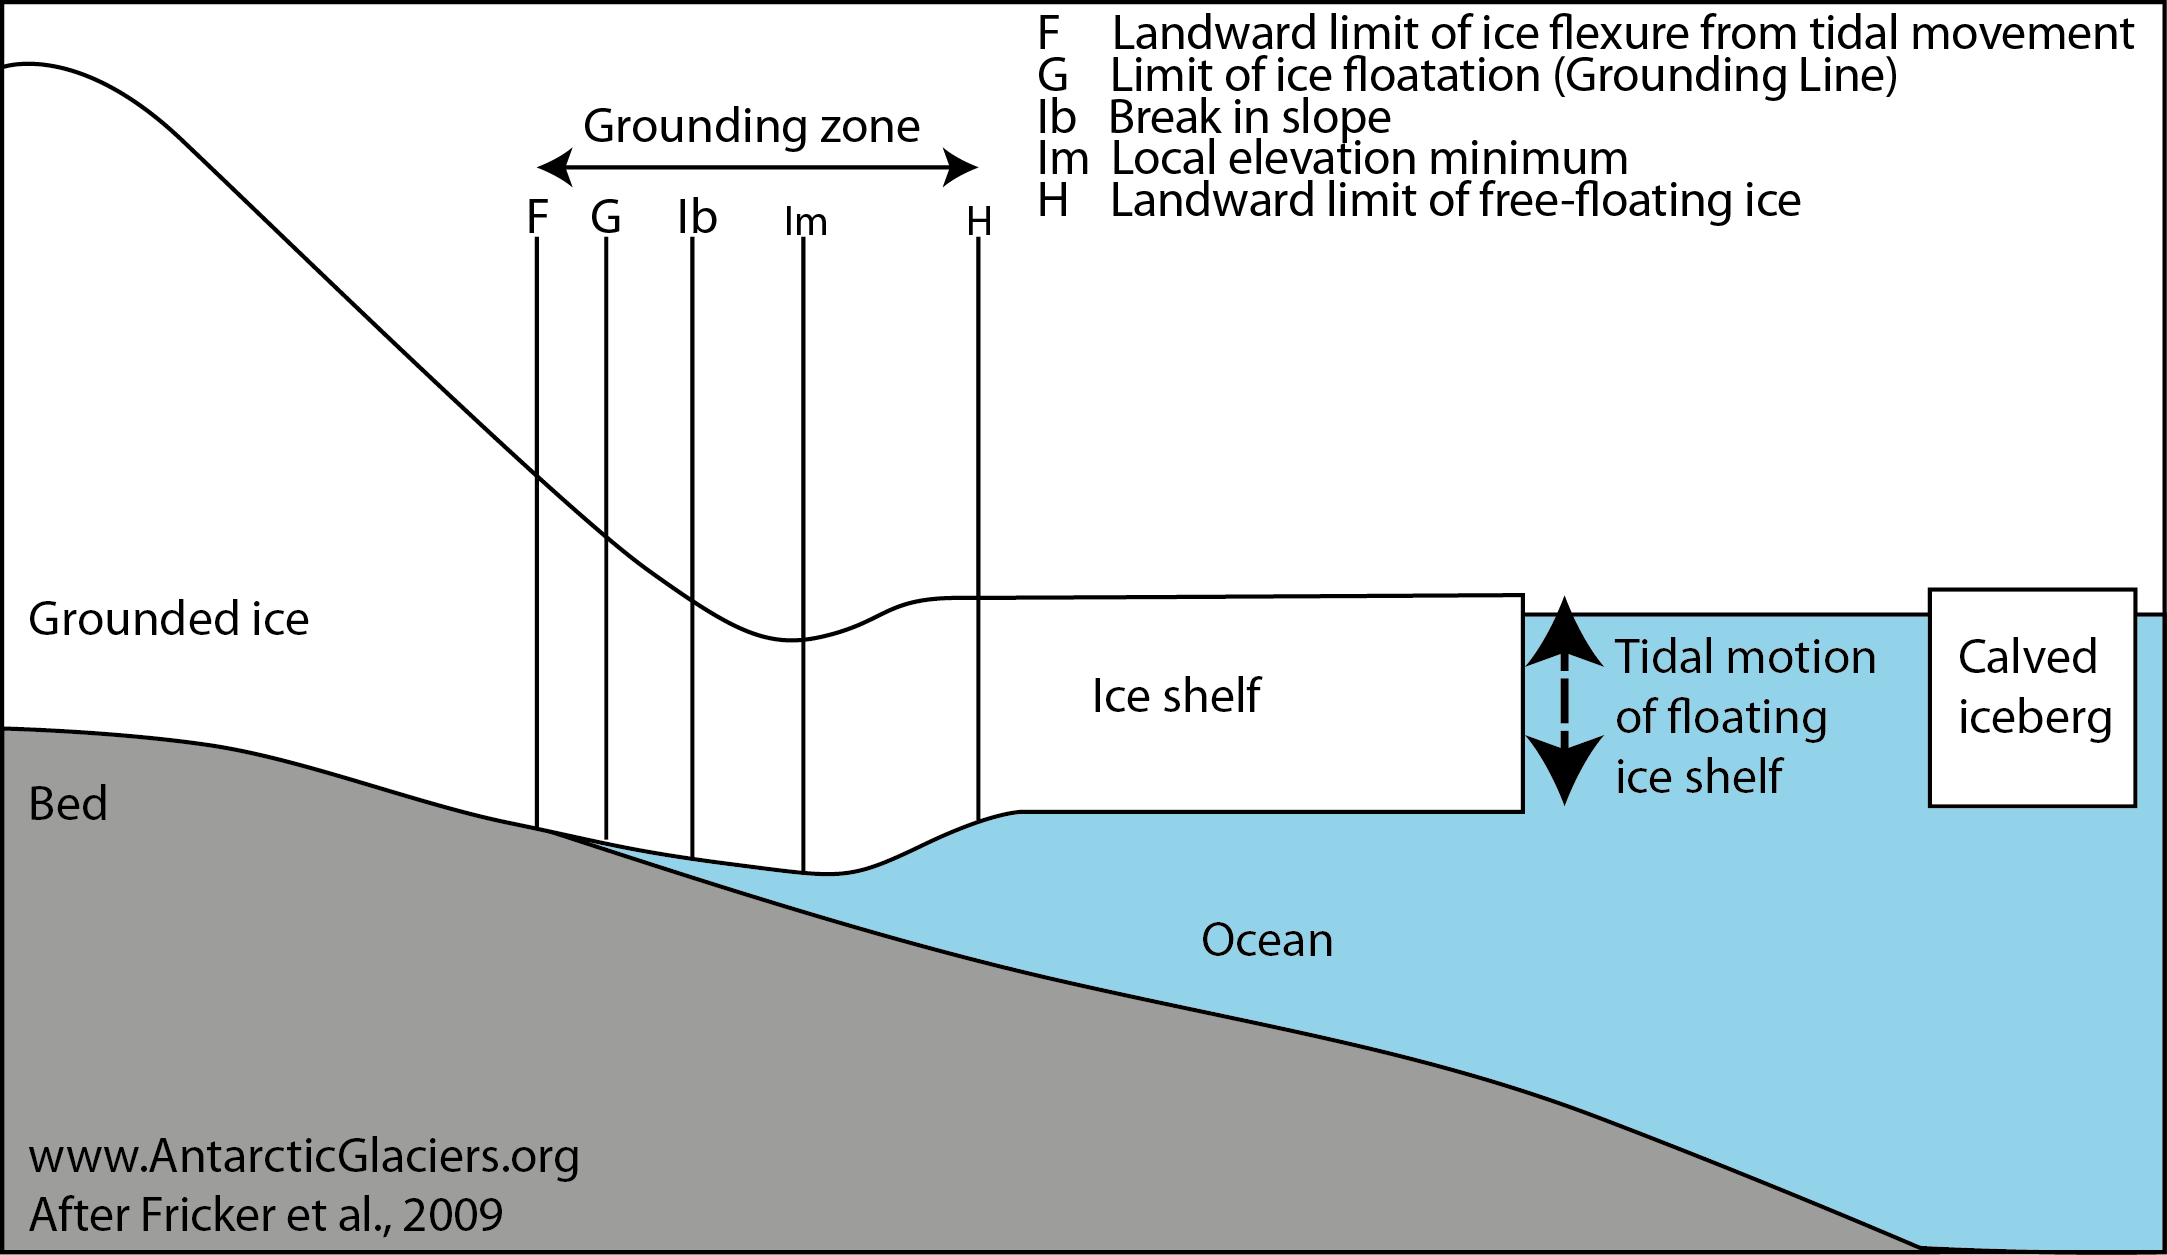
\includegraphics[scale=0.4]{../fig/groundingzone.png}
		\caption{Schema of a tributary glacier where we can observe the different parts denoting the grounding zone. Adapted from \cite{fricker2009mapping}. }
		\label{Glacier}
		\end{figure}
		\end{frame}

	\subsection{Importance of understanding the dynamics of the grounding line}
		\begin{frame}{Importance of understanding the dynamics of glaciers}
		\justifying
		\begin{itemize}
			\item The rate of present-day sea-level rise has increased in recent decades and it is expected to continue increasing in coming decades and centuries \cite[]{clark2015recent}. \pause
			\item Mass loss from glaciers is strongly linked to changes in the ice shelves and their grounding lines \cite[]{brunt2010mapping, pritchard2012antarctic}. \pause
			\item Ice thinning and rising sea levels can cause grounding line to retreat while thickening or declining sea levels can cause an advance \cite[]{friedl2020remote}.
		\end{itemize}
		\end{frame}
	\section{Glacier dynamics}
	\subsection{Glacier flow}
		\begin{frame}{Glacier flow}
		\justifying
			\begin{figure}
				\centering
				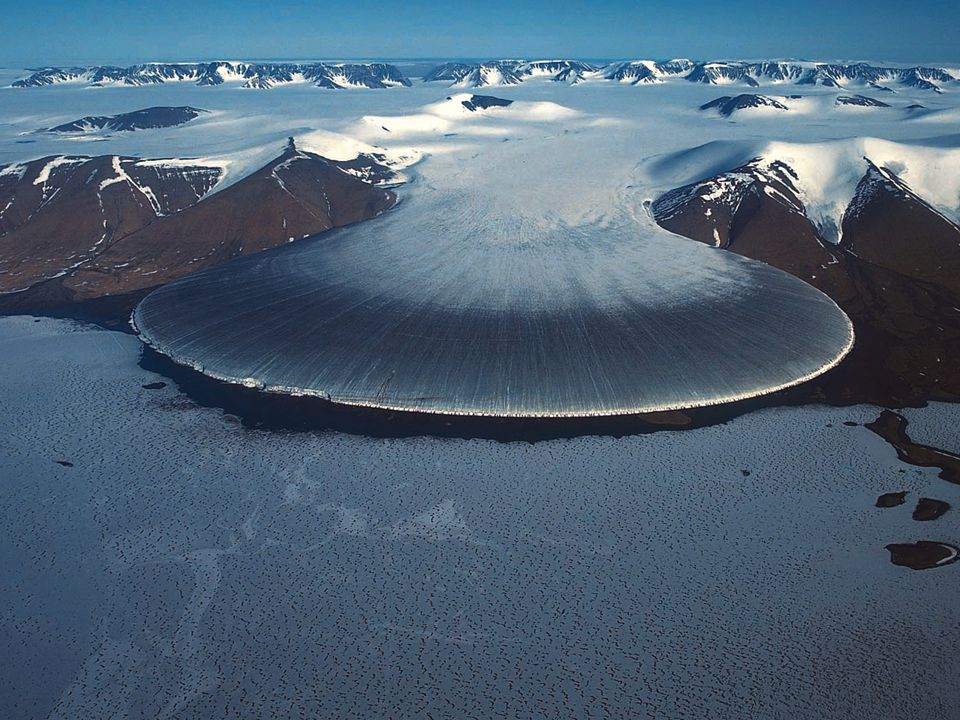
\includegraphics[scale=0.3]{../fig/glacier_flowing.png}
				\caption{Glaciers behave as a very viscous fluid for time scales between a few years to a few thousands of years. }
				\label{Flow_ice}
			\end{figure}
		\end{frame}
	\subsection{Governing equations}
		\begin{frame}{Governing equations}
		The plastic lower ice of the glacier can flow like a very viscous fluid. The incompressibility condition leads to: 
		\begin{equation}
			\nabla \cdot u=0.
		\end{equation}
		\pause For ice flow, the acceleration term can be neglected in the Navier-Stokes equations \cite[]{hutter1982mathematical}. Therefore:
		\begin{equation}
			-\nabla \cdot p+\nabla \cdot (\eta (\nabla \cdot u+(\nabla \cdot u)^T))+\rho g = 0.
		\end{equation}
		Where $\eta$ is the viscosity and $g$ is the gravity.
		\pause Letting $\sigma$ denote the stress tensor and pressure $p$ is the mean normal stress, and the strain rate tensor $\epsilon_{e}$, related by:
		\begin{equation}
			\sigma=2\eta \epsilon_{e}-pI = \eta \cdot(\nabla \cdot u+(\nabla \cdot u)^T)-pI.
		\end{equation}
		Where I is the identity tensor. Together, these two last mathematical equations are called the full-stokes model.
		
		\end{frame}
	\subsection{The flow law}
		\begin{frame}{The flow law}
			\justifying
			The most commonly used flow law for ice is Glen’s flow law, named after John W. Glen upon whose experiments it is based \cite{glen1958flow}. This equation was originally written in the form:
			\begin{equation}
				\dot{\epsilon_{e}}=({\frac{\sigma_{e}}{B}})^n;
			\end{equation}
			\pause where B is a viscosity parameter that increases as the ice becomes stiffer, and n is an empirically determined constant, and n=3. An alternative form of the flow law that is commonly used, and that can be used, is:
			\begin{equation}
				\dot{\epsilon_{e}}=A{\sigma_{e}}^n
			\end{equation}
			\pause A is called the rate factor. B is normally given in Mpa yr$^{\frac{1}{n}}$ while A is in MPa$^{-n}$ yr $^{-1}$ or MPa$^{-n}$ s $^{-1}$.
		\end{frame}
	\subsection{Boundary conditions and time evolution}
		\begin{frame}{Boundary conditions and time evolution}
		\justifying
			\begin{itemize}
				\item Ice in contact with the bedrock: Weertman sliding law \cite[]{weertman1974stability}:
				\begin{equation}
					u_b=C{\tau_b}^m;
				\end{equation}
				\pause \item The ice surface is assummed stress free $\sigma .n=0$ and ice base at $z_s$ and $z_b$ behave as free surfaces according to:
				\begin{equation}
					\frac{\delta z_{i}}{\delta t}+u_{i}\frac{\delta z_{i}}{\delta x}+v_{i}\frac{\delta z_{i}}{\delta y}=w_{i}+a_{i};
				\end{equation}
			where $a_{i}$ is the accumulation ($a_{i}>0$) or ablation ($a_{i}<0$) in meter ice equivalent per year, and $i=$ surface or base, respectively.
			\pause \item By vertical integration of the incompressibility condition, $w$ can be eliminated:
			\begin{equation}
				\frac{\delta H}{\delta t}+\frac{\delta H\bar{u}}{\delta x}+\frac{\delta H \bar{v}}{\delta y}=a_s-a_b ;
			\end{equation}
			Where $\bar{u}$ and $\bar{v}$ are the vertically integrated horizontal velocities. 
			\pause \item For the ice-ocean interface, the ice flux out of the domain will be fixed as the calving rate.
			\end{itemize}
		\end{frame}

	\subsection{Shallow shelf approximation}
		\begin{frame}{Shallow shelf approximation}
			\justifying
			SSA approximation has been derived by dimensional analysis based on a small aspect ratio between vertical and longitudinal lenght of the ice shelf
			The conservation of momentum simplifies to:
			\begin{equation}
				\nabla_h \cdot(2\bar{\eta}(\dot{\epsilon_h}I))=\rho g H \nabla_h \cdot z_s;
			\end{equation}
			Where the subscript h represents the components in the x-y plane and $\bar{\eta}$ the vertically integrated viscosity. The effective strain rate simplifies to:
			
			\begin{equation}
				\dot{\epsilon_h}=\sqrt{{\frac{\delta u}{\delta x}}^2+{\frac{\delta v}{\delta y}}^2+\frac{\delta u}{\delta x}\frac{\delta v}{\delta y}+\frac{1}{4}{(\frac{\delta u}{\delta y}+\frac{\delta v}{\delta y})}^2};
			\end{equation}

		\end{frame}
			
		
	\section{Grounding line dynamics and stability}
		\begin{frame}{Grounding line dynamics and stability}
		\begin{figure}
			\centering
			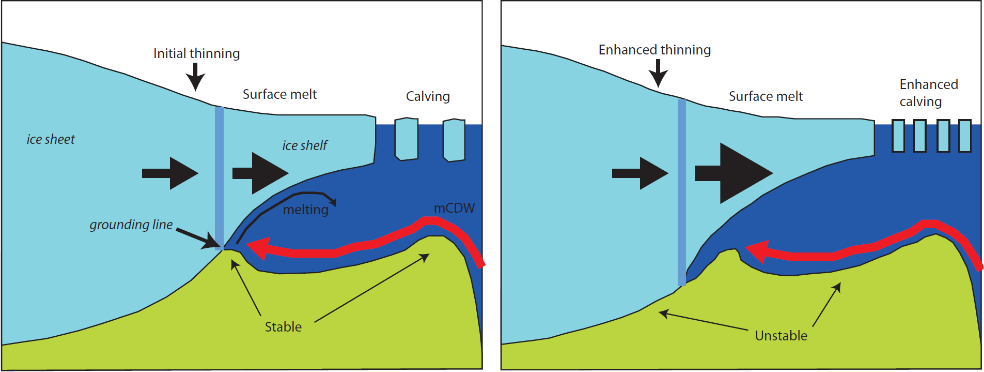
\includegraphics[scale=0.3]{../fig/GroundingLineInstability.png}
			\caption{Schematic representation of the marine ice sheet instability with an initial stable grounding line position (left hand side) and unstable grounding line position after the incursion of warm circumpolar deep water below the ice shelf. Adapted from \cite{hanna2013white}.}
			\label{grounding_line_instability}
		\end{figure}
		\end{frame}

	\section{Numerical model}
	\subsection{Process of modelling}
	\begin{frame}{Process of modelling}
		\justifying
		The physical phenomena that impacts the dynamics of the glaciers can be represented using mathematical models that implement partial differential equations, which can then be discretized to be solved using numerical methods.
		\begin{figure}
			\centering
			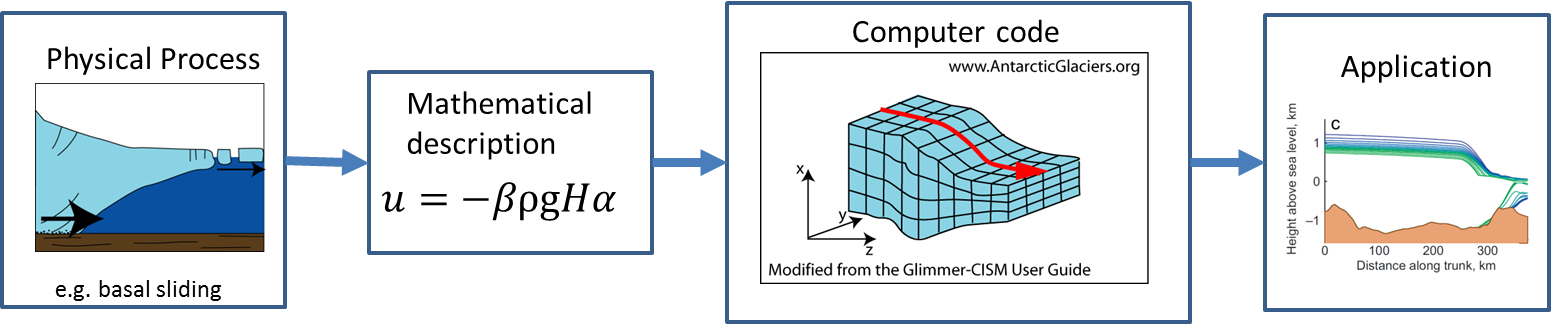
\includegraphics[scale=0.4]{../fig/Numerical_modelling_scheme.png}
			\caption{Process of modelling, starting with a physical phenomena which can be represented mathematically in a physical model than can then be discretized to solve numerically.}
			\label{Modelling}
		\end{figure}
	\end{frame}
	\subsection{Finite element methods}
		\begin{frame}{Finite element methods}
		
		\begin{itemize} 
			\justifying
			\item Numerical technique to calculate approximate solutions to differential equations problems.
			\begin{figure}
				\centering
				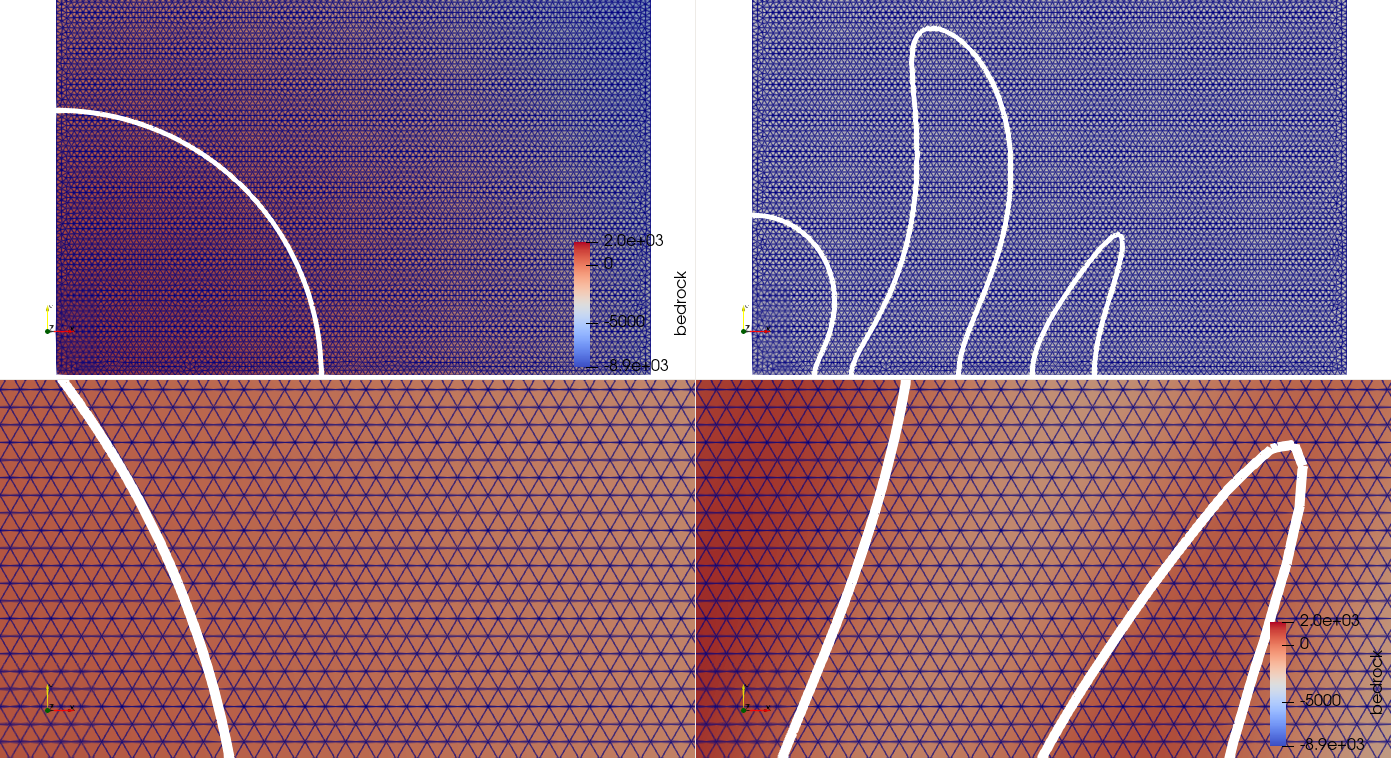
\includegraphics[scale=0.2]{../fig/grid_and_bedrock.png}
				\caption{Discretization of the glacier domain using finite elements.}
				\label{FEM}
			\end{figure}
		\end{itemize}
		\end{frame}
	\subsection{Elmer/Ice finite element method}
	\begin{frame}{Elmer/Ice finite element method}
		
		\begin{itemize}
			\justifying
			\item Open source finite element code, mainly developed in Grenoble and Helsinki. Still being developed and there are many contributors
			\pause \item The ice sheet/ice flow model Elmer/Ice is based on Elmer and includes developments related to glaciological problems. It includes a large number of dedicated solvers and users functions.
			\pause \item Elmer/Ice solves the Stokes equations and it includes solvers for the approximations of the Stokes equations, namely shallow shelf and shallow ice approximations.
		\end{itemize}
	\end{frame}
	\section{Systems and experiment set-up}
	\subsection{Calving intercomparison project CalvingMIP}
	\begin{frame}{Calving intercomparison project}
		\begin{itemize}
		\justifying
		\item The intercomparison project (https://github.com/JRowanJordan/CalvingMIP) is intended to develop models to explore calving, ice damage, and glacier dynamics leading to recommendations for improved calving laws in ice sheet models.
		\pause \item The objective is to develop a model based on the topographies proposed by the CalvingMIP project to study the grounding line position for different resolutions.
		\end{itemize}
		
	\end{frame}
	\subsection{Cone domain}
		\begin{frame}{Cone domain}
		\justifying
		The idealised experimental domain comprise a simple, symmetrically circular domain. This first idealized model consists of a circular bedrock configuration (Figure \ref{circular_topo_top}) given by:
		\begin{equation}
			Bed_0=Bc-(Bc-BI)\frac{|x^2+y^2|}{r^2};
		\end{equation}
		Where r=800x10$^3$m, Bc=0.9 x 10$^3$m, and BI=-2 x 10$^3$m. \pause
		\begin{figure}
			\centering
			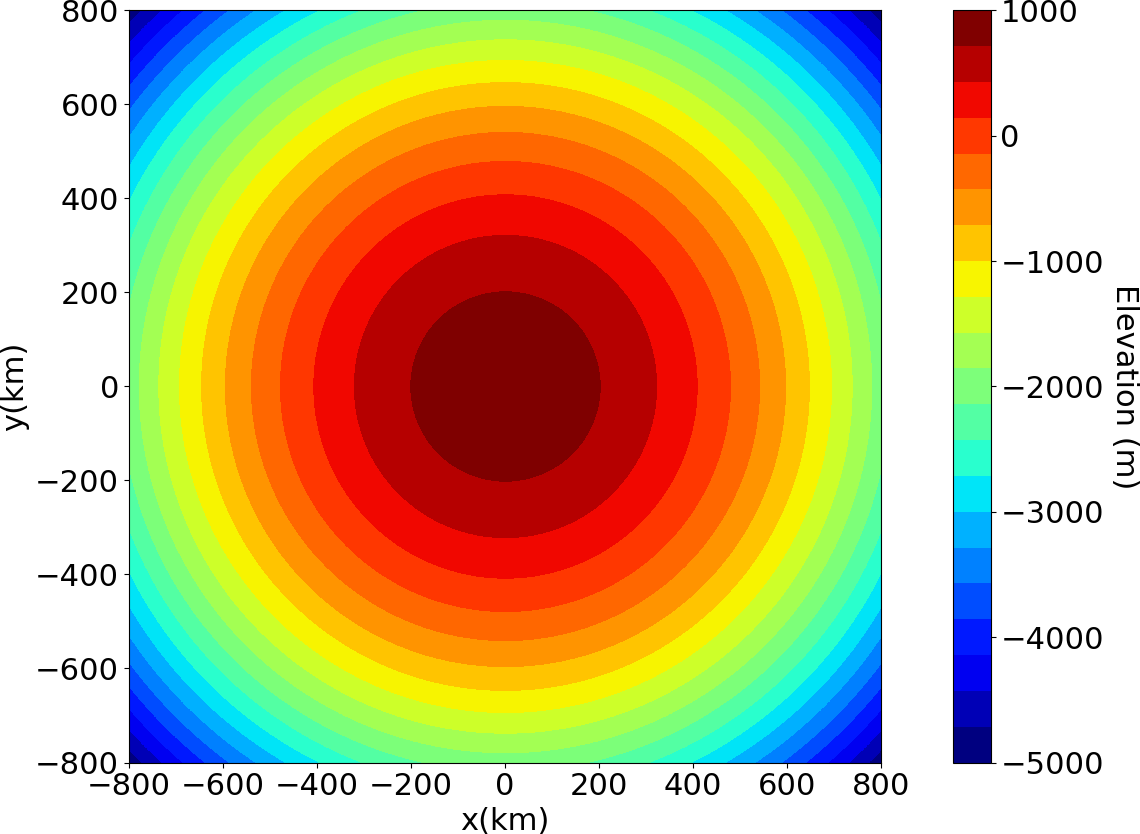
\includegraphics[width=0.45\linewidth]{../fig/circular_topo_top.png}
			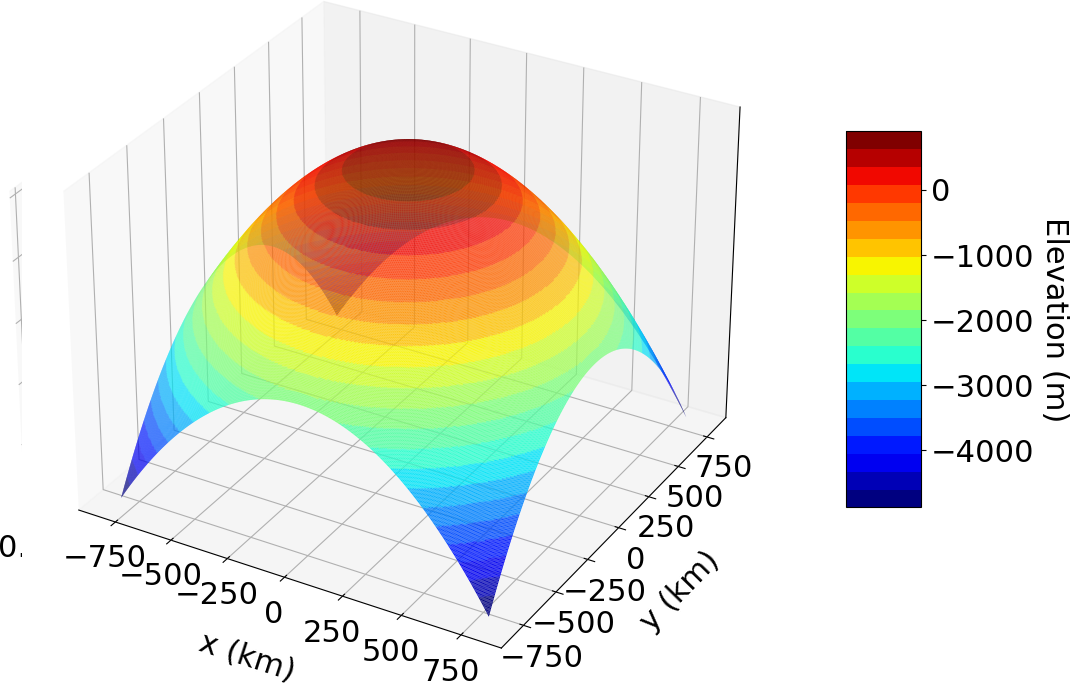
\includegraphics[width=0.45\linewidth]{../fig/circular_topo_jet}
			\caption{Circular bedrock topography. On the left side top view and on the right side, lateral view.}
			\label{circular_topo_top}
		\end{figure}
		\end{frame}
		\begin{frame}{Experimental profiles}
		\begin{figure}
			\centering
			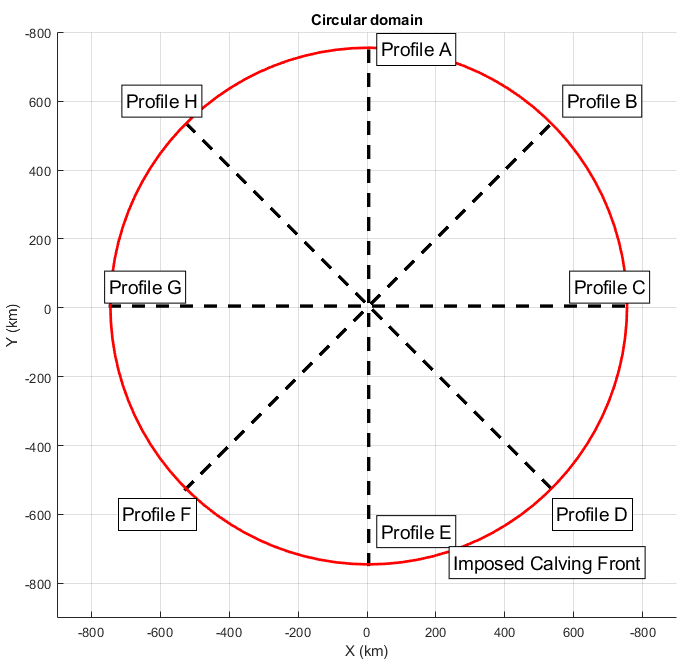
\includegraphics[width=0.5\linewidth]{../fig/cone.png}
			\caption{Circular domain experimental profiles as well as the initial imposed calving front position. Adapted from CalvingMIP inter-comparison project.}
			\label{cone_profile}
		\end{figure}
		\end{frame}
	
	\subsection{Thule domain}
		\begin{frame}{Thule domain}
			The Thule bedrock configuration is shown in Figure \ref{Thule_3D} and is given by:
			\begin{equation}
				\theta=arctan2(y,x);
			\end{equation}
			\begin{equation}
				I=r-cos(2\theta)\frac{r}{2};
			\end{equation}
			\begin{equation}
				Bed_0=Bc-(Bc-BI)\frac{|x^2+y^2|}{r^2};
			\end{equation}
			\begin{equation}
				Bed=Bacos(3\pi\frac{\sqrt{x^2+y^2}}{I})+Bed_0;
			\end{equation}
			With r=800 x 10$^3 m$, Bc=0,9 x 10$^3 m$, BI=-2 x 10$^3 m$, and Ba=1.1 x 10$^3 m$.
		\end{frame}
			\begin{frame}{Thule domain bedrock topography}
			\begin{figure}
				\centering
				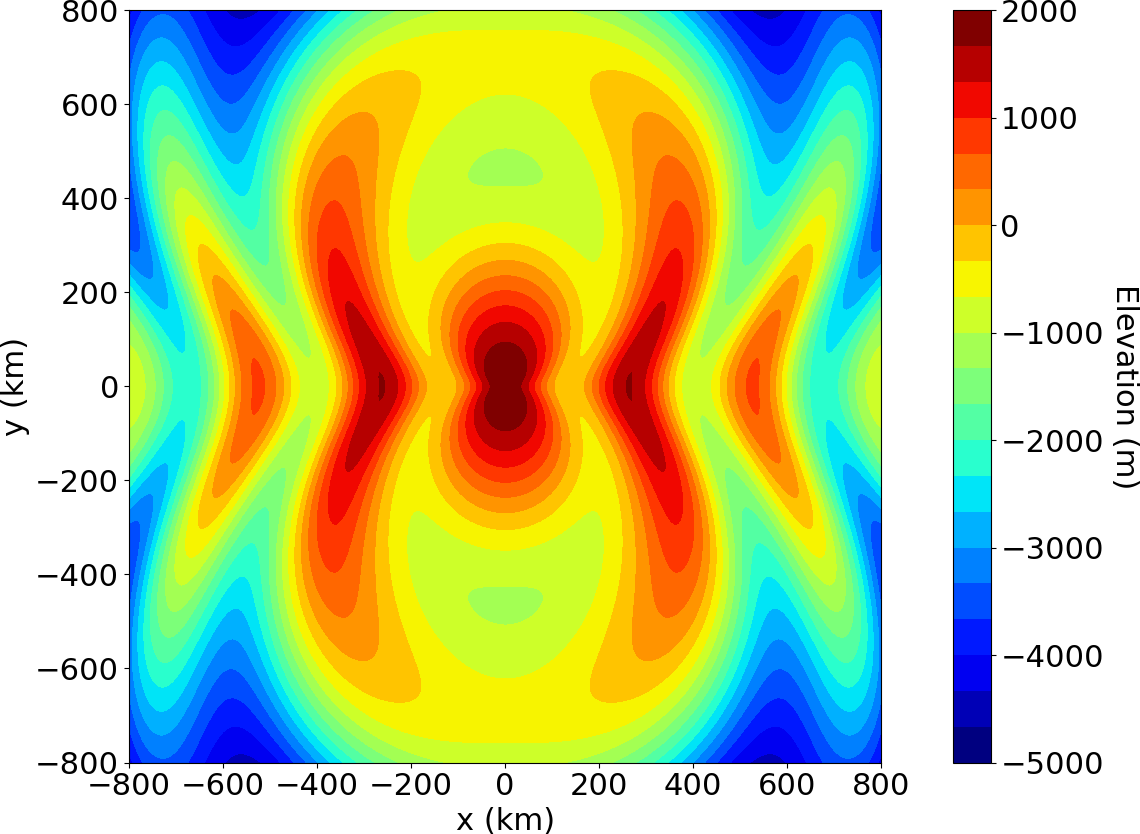
\includegraphics[width=0.45\linewidth]{../fig/Thule_2D}
				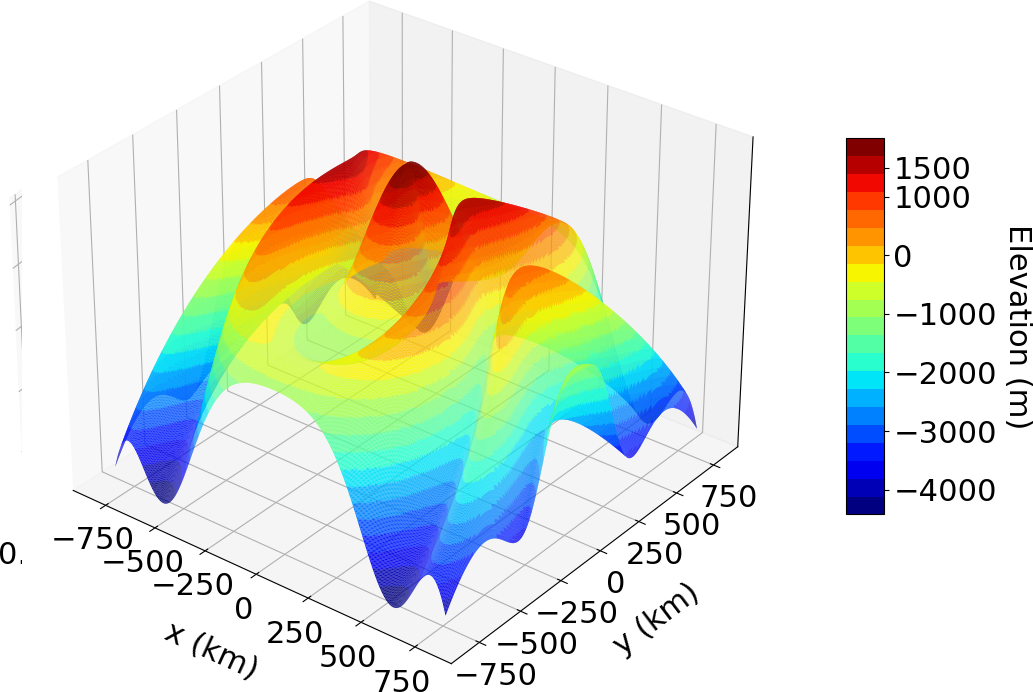
\includegraphics[width=0.45\linewidth]{../fig/Thule_3D}
				\caption{Thule bedrock topography 3D. On the left side the top view, and on the right side a lateral view.}
				\label{Thule_3D}
			\end{figure}
			\end{frame}
			\begin{frame}{Thule experimental profiles}
			\begin{figure}
				\centering
				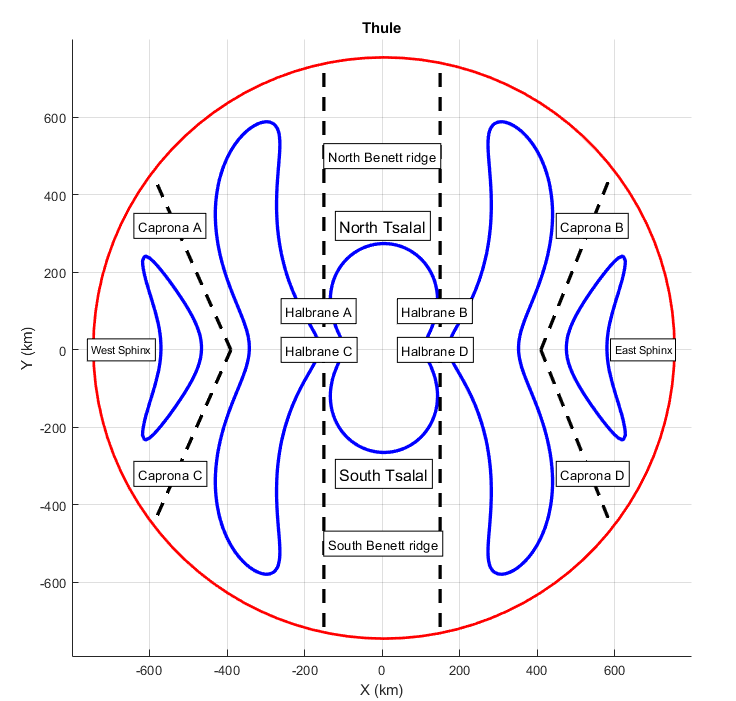
\includegraphics[width=0.5\linewidth]{../fig/thule.png}
				\caption{Thule domain experimental profiles as well as the initial imposed calving front position. Adapted from CalvinMIP inter-comparison project.}
				\label{thule_profile}
			\end{figure}
			\end{frame}
		
\section{Numerical parameters}
	\begin{frame}{Numerical parameters}
		\justifying
		\begin{table}
			\begin{center}
				\caption{Physical parameters}
				\label{Physical constants}
				\begin{tabular}{|l|l|l|}
					\hline
					Variable          & Description                 & Units           \\ \hline
					$g=9.81$         & Gravitational acceleration  & ms$^{-2}$         \\ \hline
					$a_s=0.3$       & Surface mass balance (SMB)  & ma$^{-1}$         \\ \hline
					$a_b=0$             & Basal mass balance (BMB)    &   ma$^{-1}$         \\ \hline
					$\rho i=917$        & Ice density                 & kg m$^{-3}$       \\ \hline
					$\rho w=1028$      & Sea water density           & kg m$^{-3}$       \\ \hline
					$A= 2.9377$x$10^{-9}$ & Ice rate factor             & KPa$^{-3}$a$^{-1}$  \\ \hline
					$n=3$               & Flow law stress exponent    &  Dimensionless               \\ \hline
					$C=0.001$           & basal slipperiness          & ma$^{-1}$KPa$^{-3}$ \\ \hline
					$m=3$               & Sliding law stress exponent &   Dimensionless              \\ \hline
					$s2a=31556926$     & Seconds in a year           & s         \\ \hline
				\end{tabular}
			\end{center}
		\end{table}
	\end{frame}
	\subsection{Numerical variables, external forcings and initial condition}
	\begin{frame}{Numerical variables, external forcings and initial condition}
		\begin{itemize}
			\item The numerical resolution will be the variable parameter, varying from 10km, 5km, 2km, and 1km.
			\pause \item The external forces acting will be gravity, as well as the ice friction and the basal stress.
			\pause \item The initial condition will be a topography with no ice, namely $h_0$=0m.
			\pause \item The CFL condition will be necessary to verify the stability of the model. It is needed that:
			\begin{equation}
				C=\frac{u\Delta t}{\Delta x}<C_{max};
			\end{equation}
			where, C is the Courant number, $u$ is the velocity, $\Delta t$ is the time step, $\Delta x$ is the horizontal resolution. C$_{max}=1$ is a safe approximation.  
		\end{itemize}
	\end{frame}
	\section{Results}
		\begin{frame}{Results:Cone ice thickness}
		\justifying
		\begin{figure}
			\centering
			\begin{subfigure}{.5\textwidth}
				\centering
				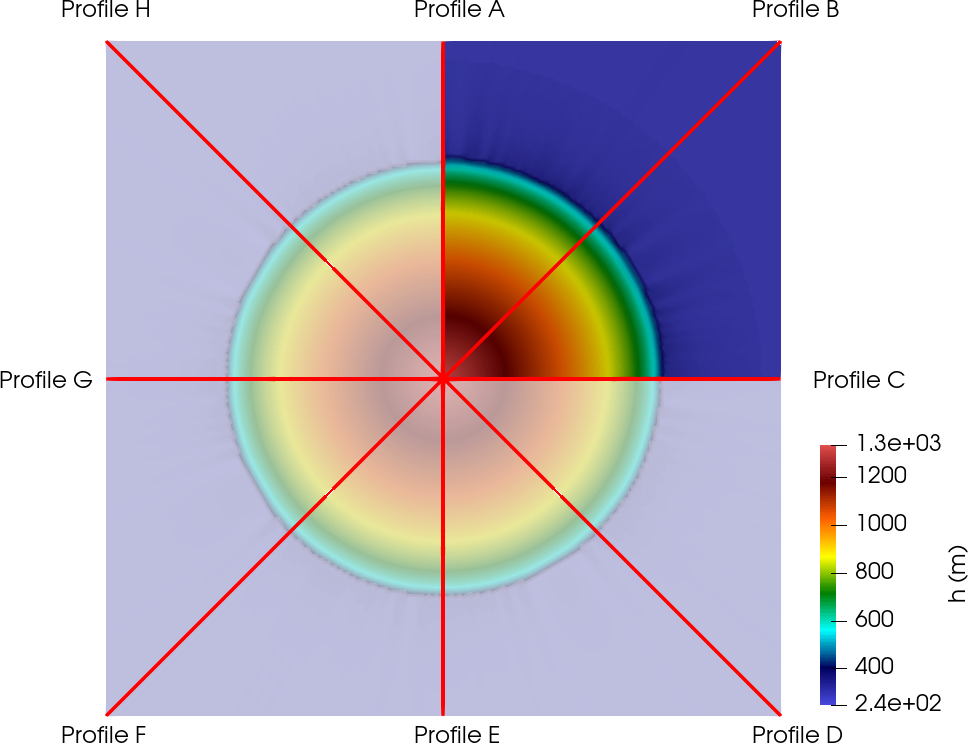
\includegraphics[width=0.99\linewidth]{../fig/Profiles_Cone_combined_domains.png}
				\caption{Profiles for Cone circular domain}
				\label{Schematic_Cone}
			\end{subfigure}%
			\begin{subfigure}{.5\textwidth}
				\centering
				\includegraphics[width=0.99\linewidth]{../fig/Profiles_Cone_domain_sin_fondo.png}
				\caption{Ice thickess per profile}
				\label{Profiles_cone}
			\end{subfigure}
			\caption{Circular domain ice sheet showing the ice thickness results along the profiles proposed.}
			\label{Cone_scheme}
		\end{figure}
		\end{frame}
		\begin{frame}{Volume variation in time and per number of nodes}
		\begin{figure}
			\centering
			\begin{subfigure}{.5\textwidth}
				\centering
				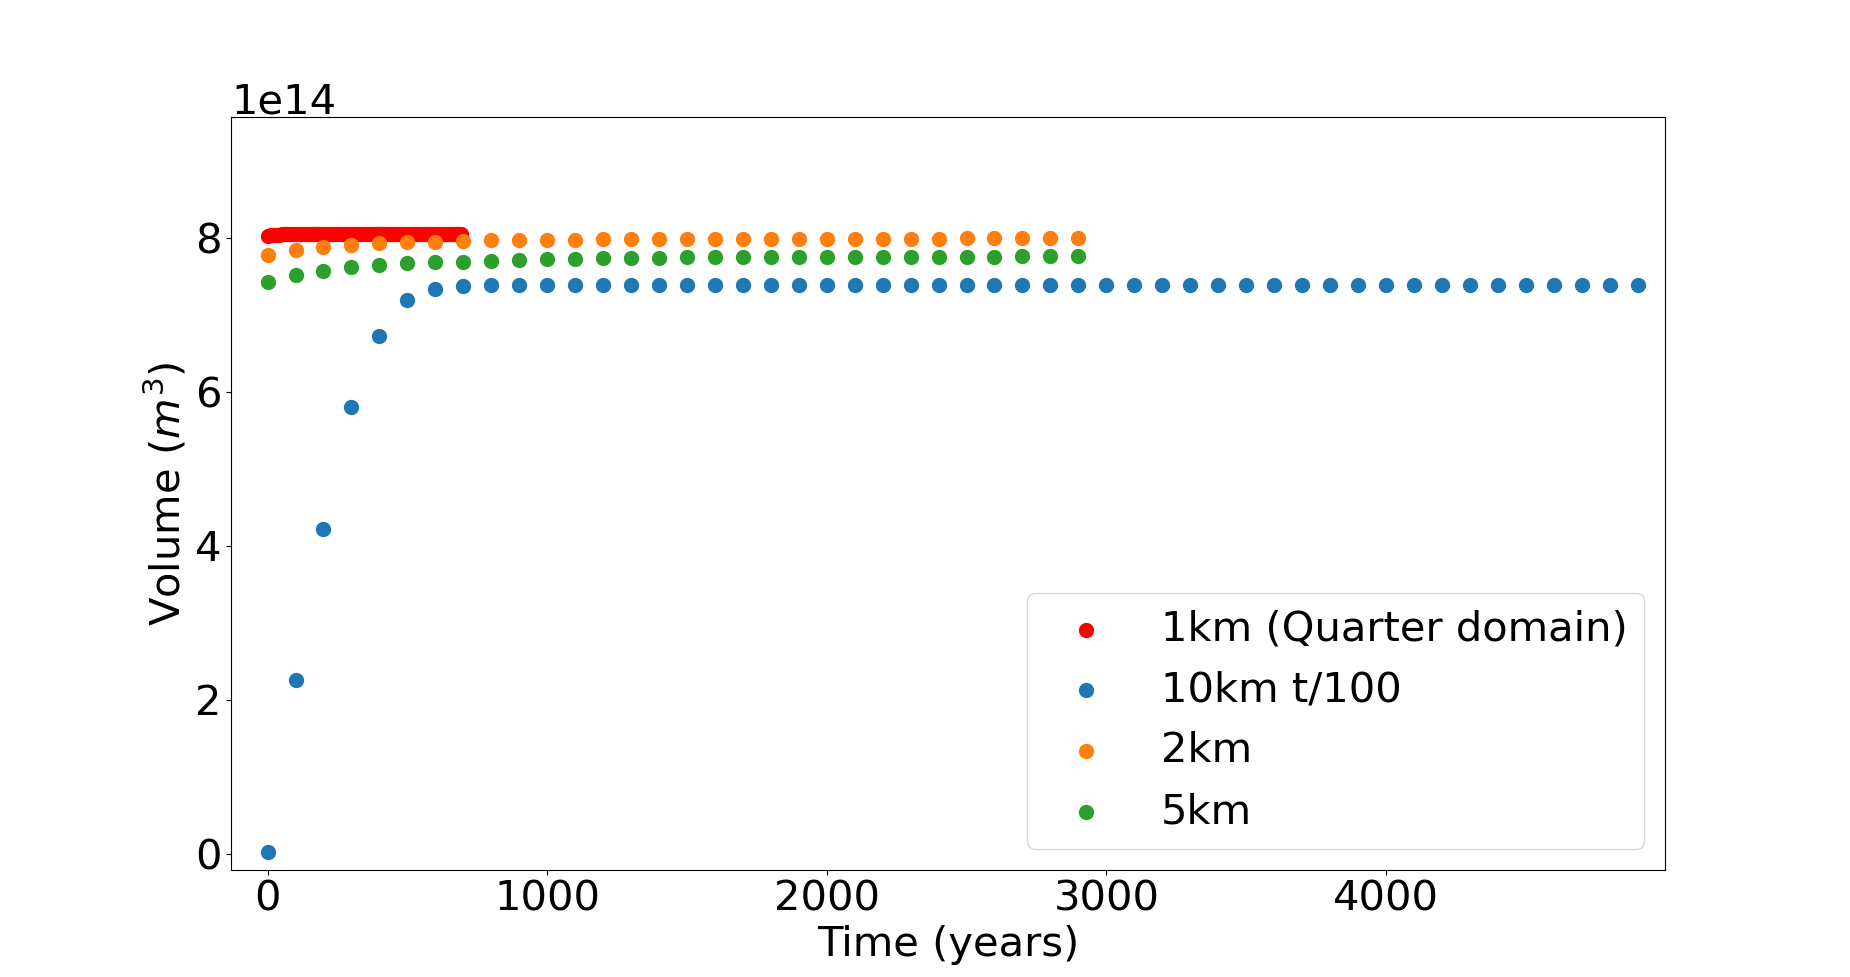
\includegraphics[width=1.1\linewidth]{../fig/Volume_CONE_full_all_res_vs_time_2.png}
				\caption{Volume variation in time.}
				\label{VOLUME_CONE_VS_TIME}
			\end{subfigure}%
			\begin{subfigure}{.5\textwidth}
				\centering
				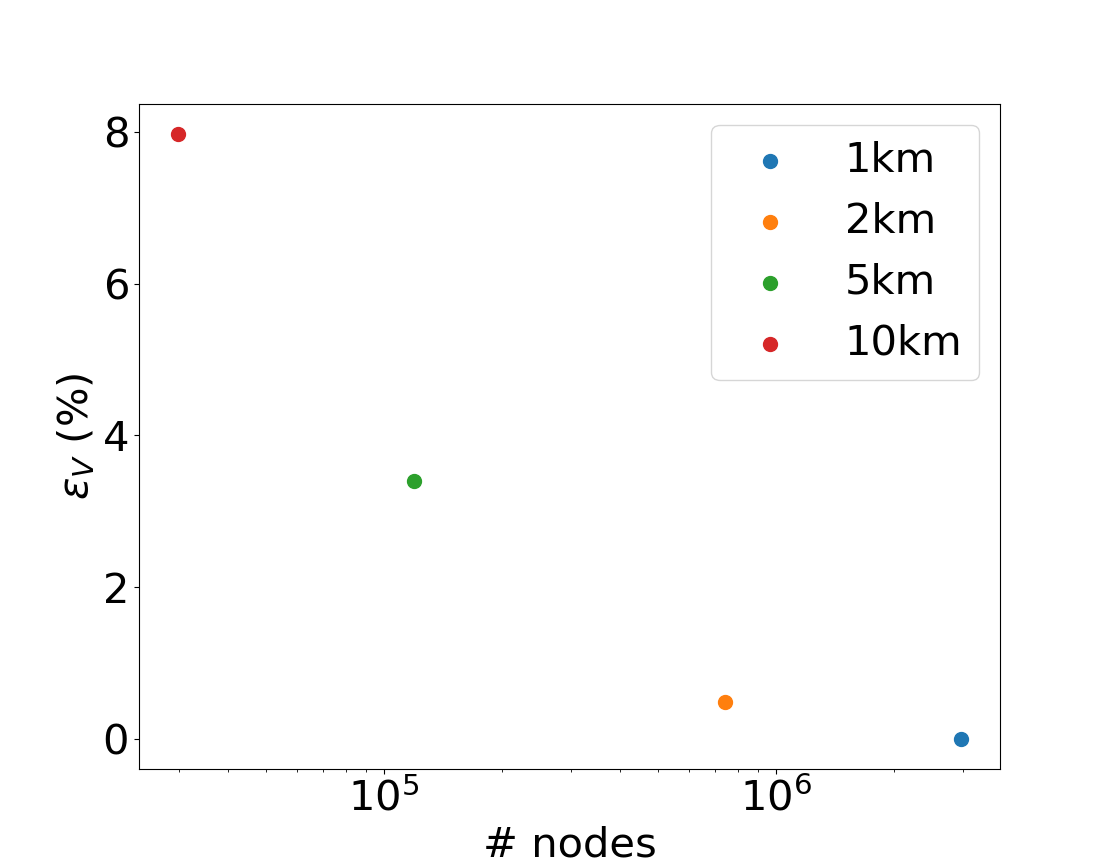
\includegraphics[width=1.1\linewidth]{../fig/Volume_CONE_full_all_res_vs_num_nodes.png}
				\caption{Volume relative variation as a function of the number of nodes.}
				\label{H_CONE_VS_NODES}
			\end{subfigure}%
			\caption{Volume variation in time and per number of nodes for the cone experiment.}
			\label{Volume_CONE_VS_TIME_VS_NODES}
		\end{figure}
		\end{frame}
		\begin{frame}{Simulations time as a function of the number of nodes}
			
	
		\begin{figure}
			\centering
			\begin{subfigure}{.5\textwidth}
				\centering
				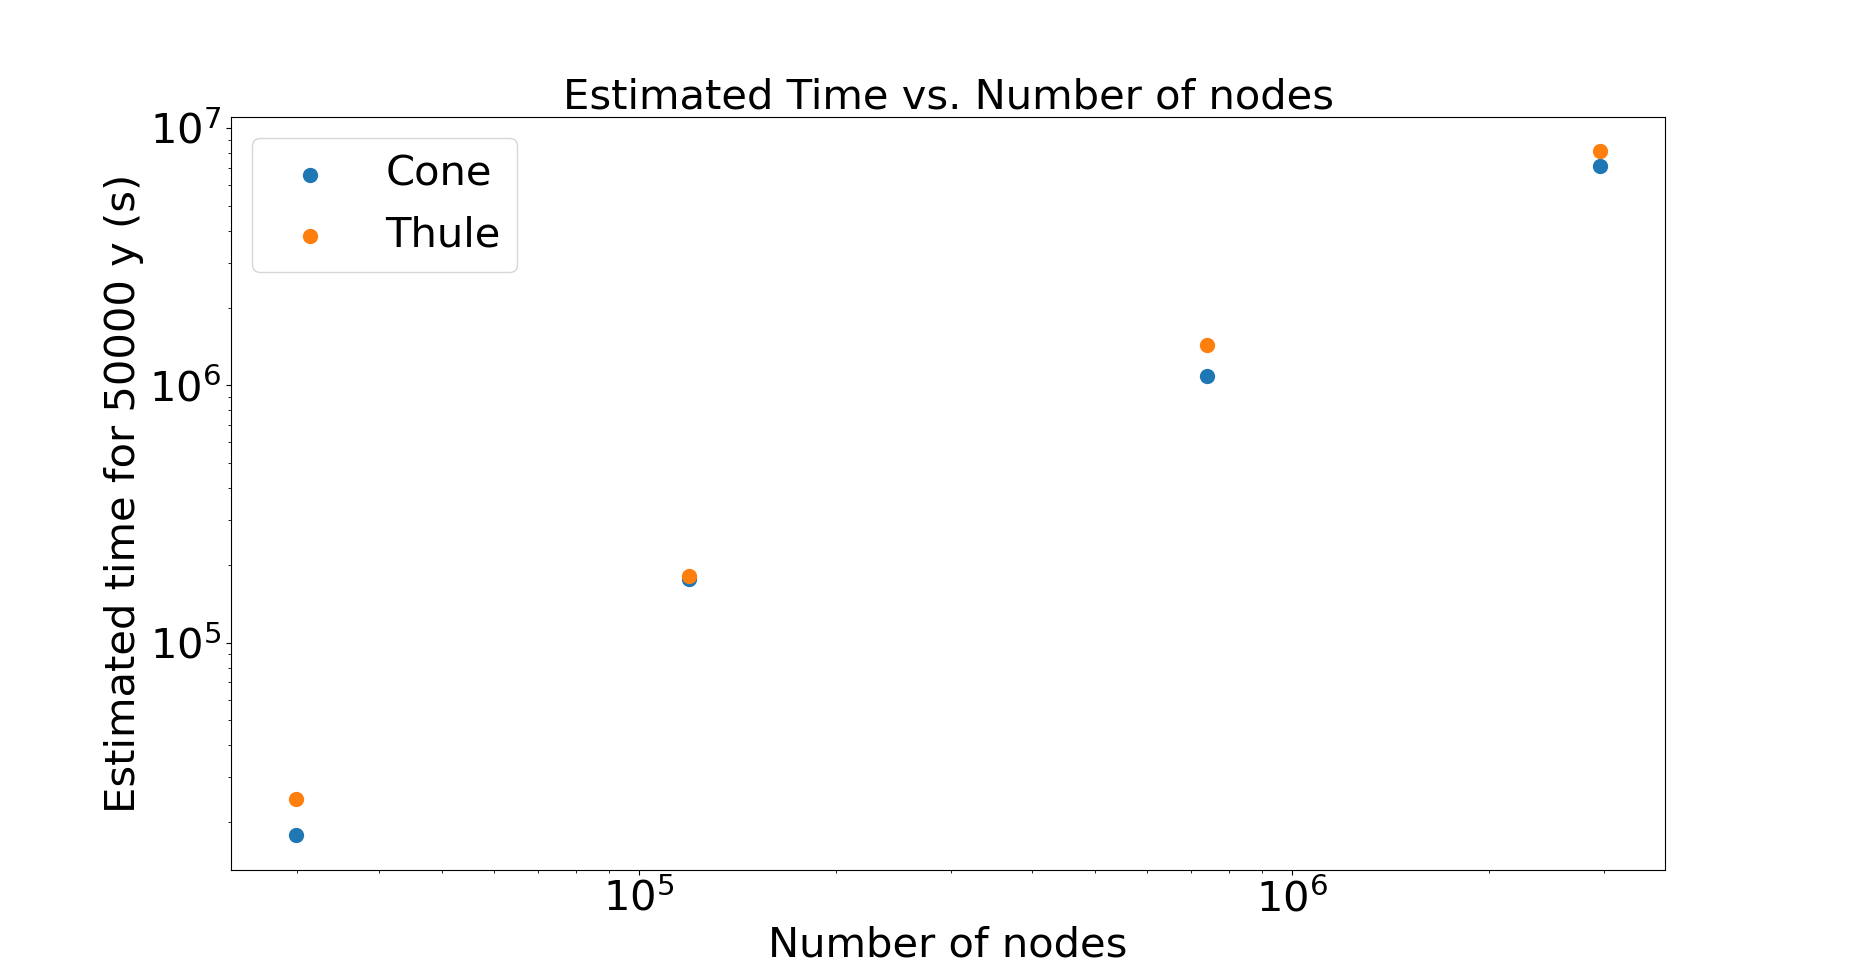
\includegraphics[width=1.1\linewidth]{../fig/Figure_Time_vs_nodes_Segundos.png}
				\caption{Time for 32 processors used.}
				\label{32_proce}
			\end{subfigure}%
			\begin{subfigure}{.5\textwidth}
				\centering
				\includegraphics[width=1.1\linewidth]{../fig/Figure_Time_vs_nodes_32.png}
				\caption{Time for 1 processor.}
				\label{1_proce}
			\end{subfigure}
			\caption{Simulation time as a function of the number of nodes for each resolution mesh.}
			\label{Computation time}
		\end{figure}
		\end{frame}
	\begin{frame}{Grounding line position per resolution}
		\begin{figure}
			\centering
			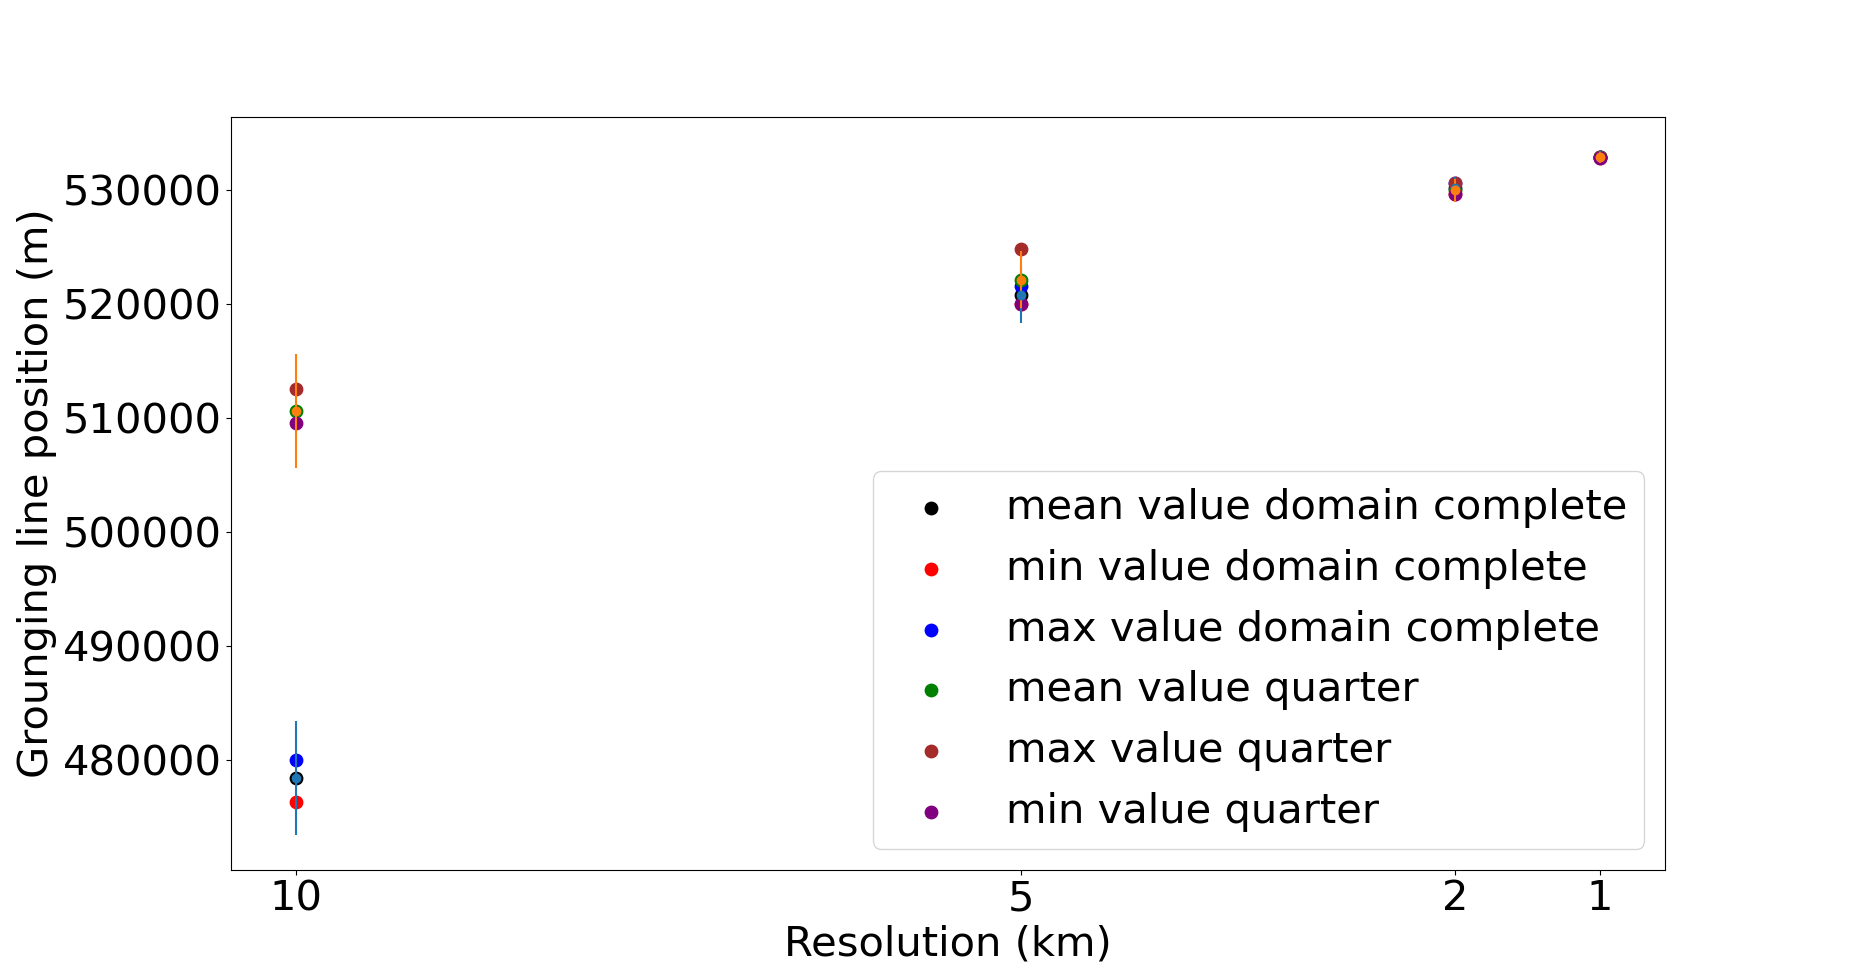
\includegraphics[width=0.8\linewidth]{../fig/Figure_CONE_GL_positions.png}
			\caption{Grounding line positions as a function of the resolution for quarter and complete circular cone domain.}
			\label{Grounding_lines__CONE_comparison}
		\end{figure}
	
	\end{frame}
	\subsection{Thule ice thickness}
		\begin{frame}{Results: Thule ice thickness}
			\justifying
			\begin{figure}
				\centering
				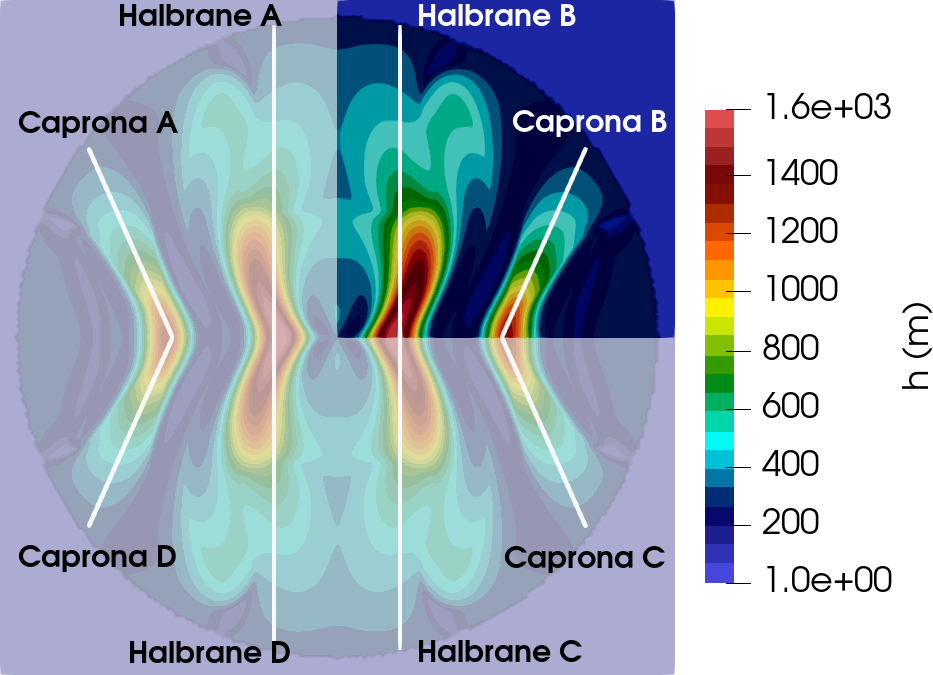
\includegraphics[scale=0.2]{../fig/Profiles_Thule_combined_domains_2_con_fondo.png}%
				\caption
				{%
					Ice thickness along the different profiles for the thule domain%
					\label{Profiles_Thule}%
				}%
			\end{figure}
		\end{frame}
		\begin{frame}{Ice thickness along profiles}
				\begin{figure}
				\centering
				\begin{subfigure}{.5\textwidth}
					\centering
					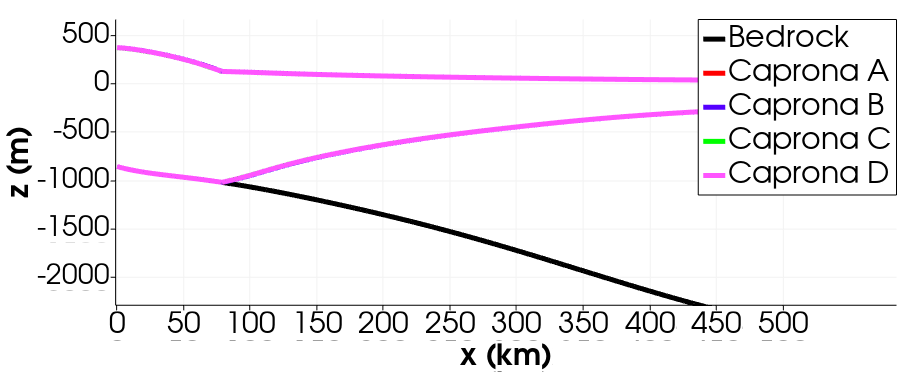
\includegraphics[width=1\linewidth]{../fig/Capronas_Thule_Domain_con_fondo.png}
					\caption{Ice thickness along each Caprona profiles.}
					\label{Capronas_thule}
				\end{subfigure}%
				\begin{subfigure}{.5\textwidth}
					\centering
					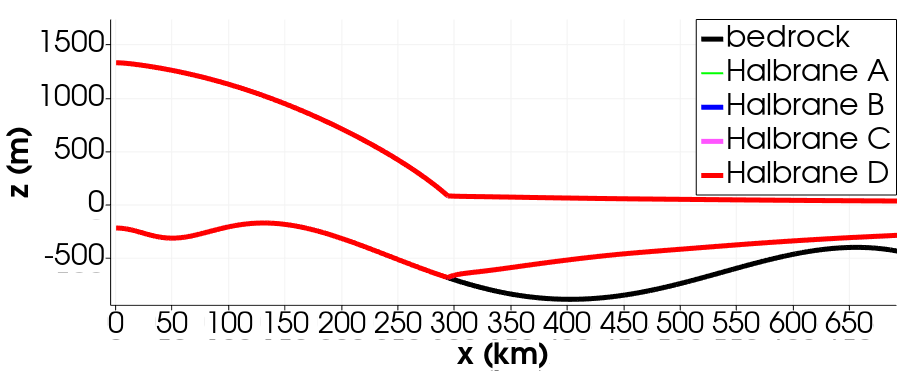
\includegraphics[width=1\linewidth]{../fig/Halbranes_thule_domain_con_fondo.png}
					\caption{Ice thickness along each Halbrane profiles.}
					\label{Halbranes_thule}
				\end{subfigure}
				\caption{Ice thickness along the thule domain profiles.}
				\label{Thule_profiles_capronas_and_halbranes}
			\end{figure}
		\end{frame}
		\begin{frame}{Volume variation in time and per number of nodes}
			\begin{figure}
				\centering
				\begin{subfigure}{.5\textwidth}
					\centering
					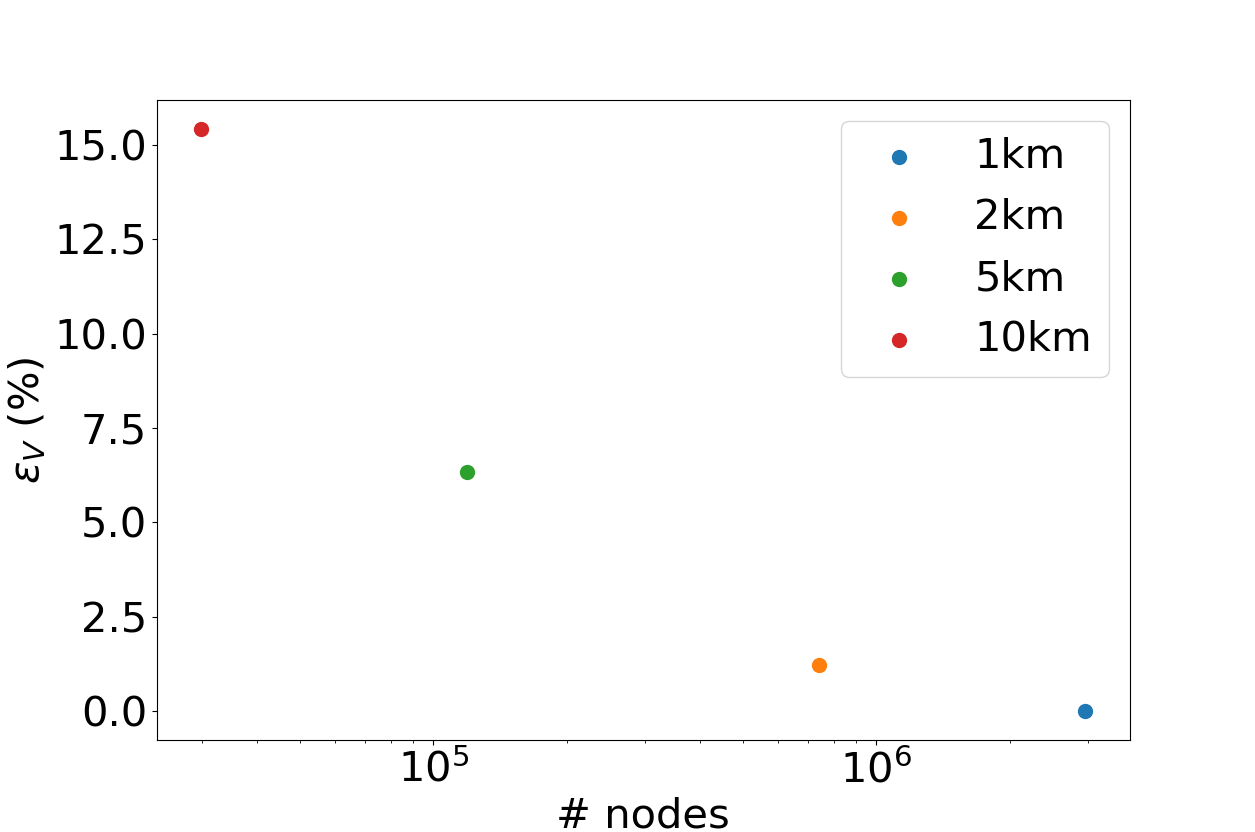
\includegraphics[width=1.1\linewidth]{../fig/Volume_THULE_full_all_res_vs_num_nodes.png}
					\caption{Volume relative variation as a function of the number of nodes.}
					\label{H_THULE_VS_NODES}
				\end{subfigure}%
				\begin{subfigure}{.5\textwidth}
					\centering
					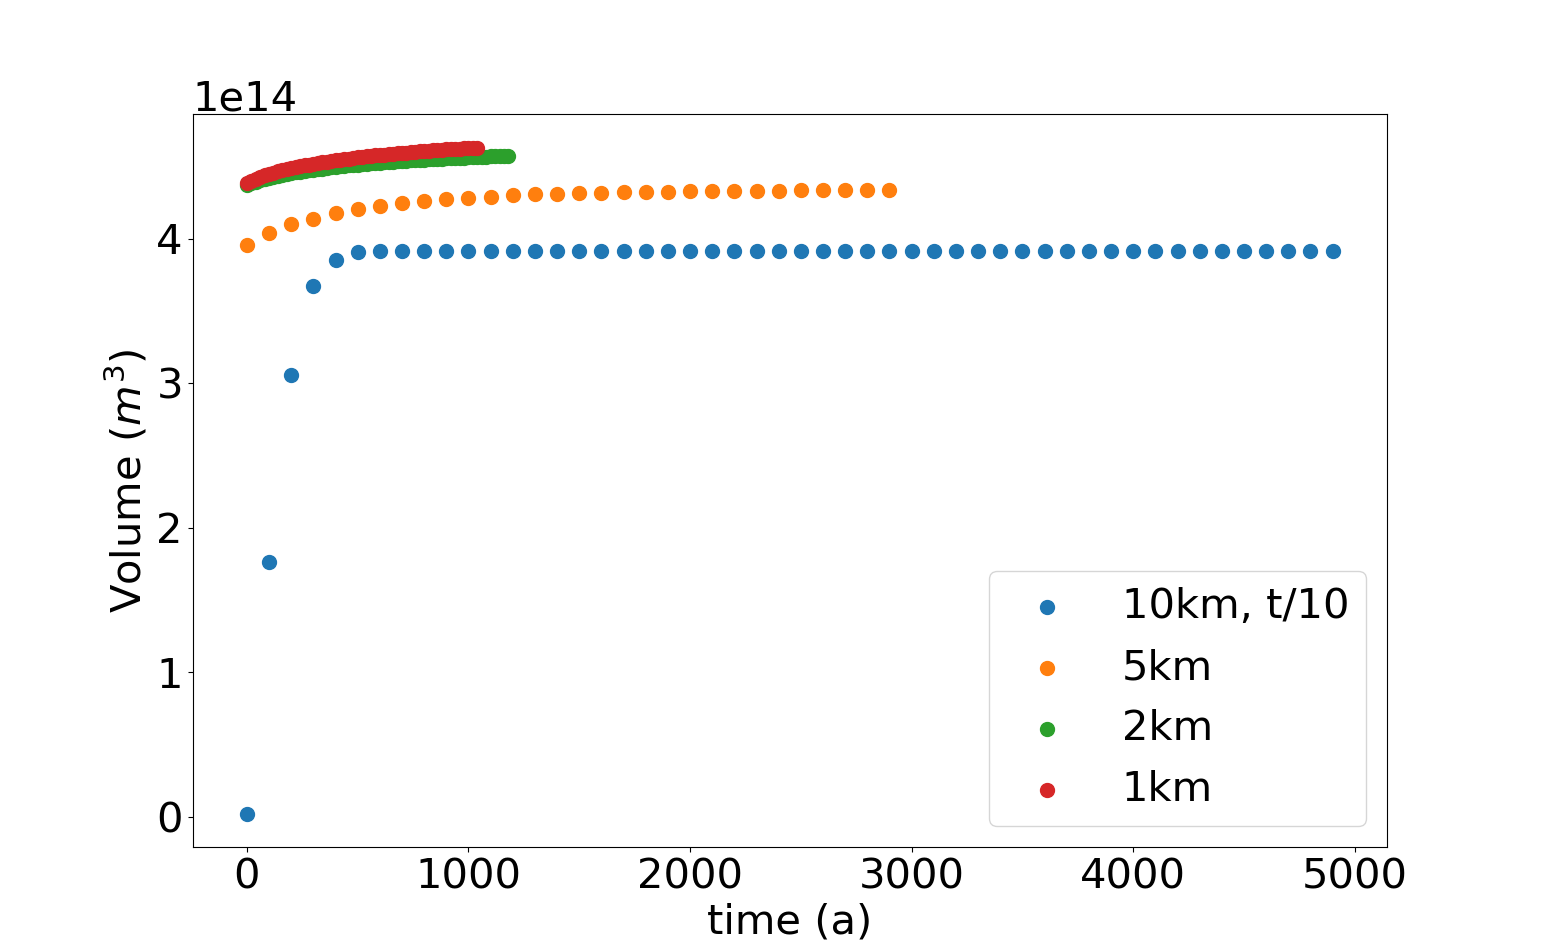
\includegraphics[width=1.1\linewidth]{../fig/Volume_THULE_full_all_res_vs_time.png}
					\caption{Volume variation in time.}
					\label{VOLUME_THULE_VS_TIME}
				\end{subfigure}
				\caption{Volume variation in time and as a function of the number of nodes for the Thule experiment.}
				\label{H_THULE_VS_TIME_VS_NODES}
			\end{figure}
		\end{frame}
		\begin{frame}{Grounding line position along profiles in Thule}
			\begin{figure}
				\centering
				\begin{subfigure}{.5\textwidth}
					\centering
					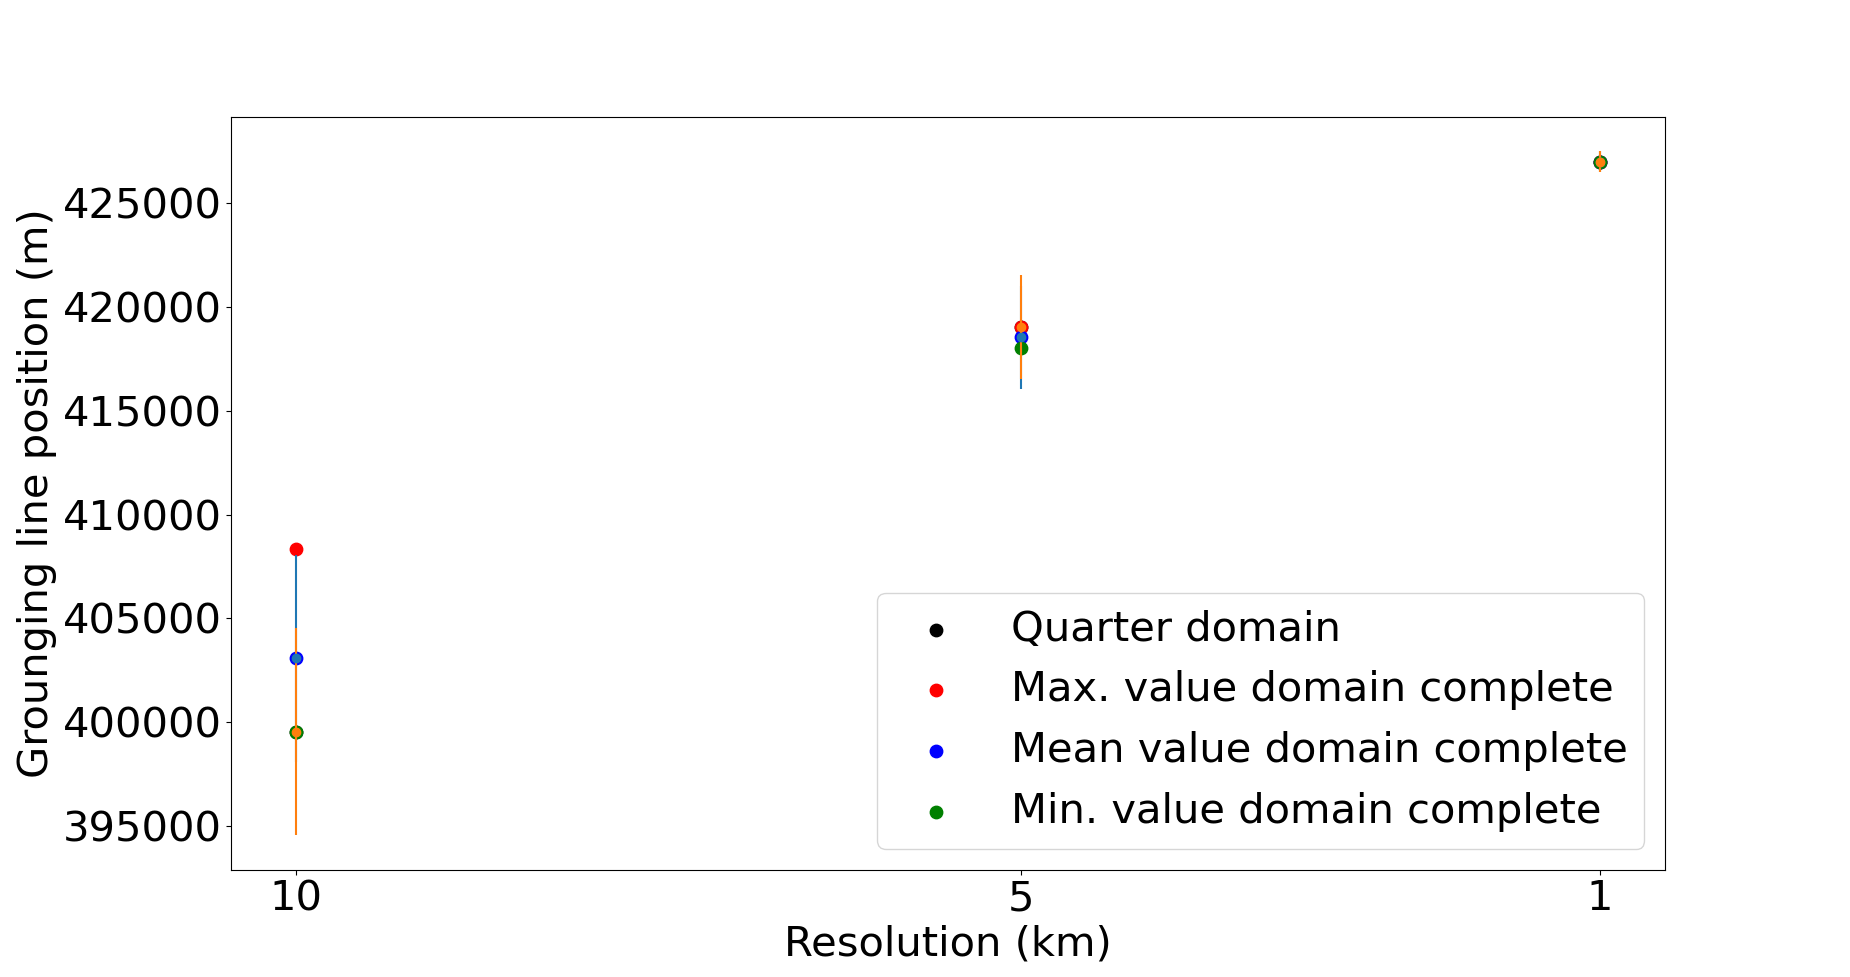
\includegraphics[width=1.1\linewidth]{../fig/Figure_THULE_GLpositions_Capronas.png}
					\caption{Grounding line positions along Capronas profiles.}
					\label{Thule_Capronas}
				\end{subfigure}%
				\begin{subfigure}{.5\textwidth}
					\centering
					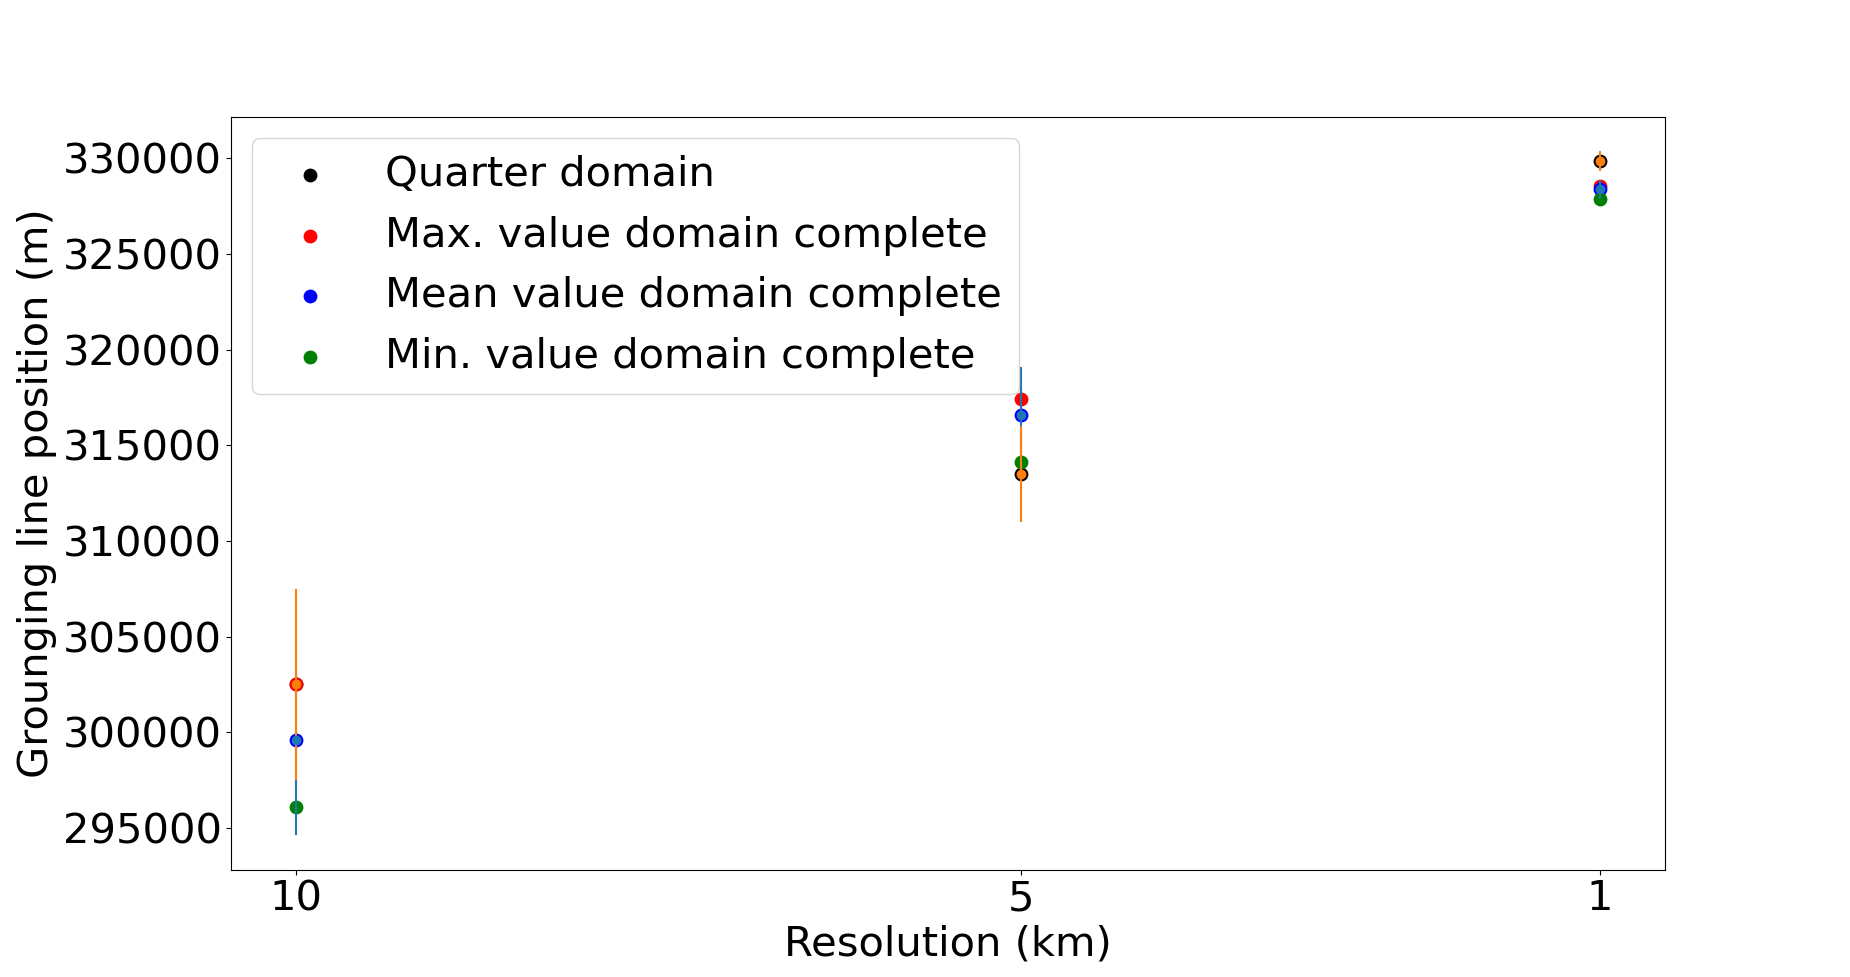
\includegraphics[width=1.1\linewidth]{../fig/Figure_THULE_GLpositions_Halbranes.png}
					\caption{Grounding line positions along Halbrane profiles}
					\label{Thule_halbranes}
				\end{subfigure}
				\caption{Grounding line positions as a function of the resolution for quarter and complete thule domain along the Caprona and Halbrane profiles.}
				\label{Grounding_lines__caprona_halbrane_comparison}
			\end{figure}
		\end{frame}
	\section{Conclusions}
		\begin{frame}{Conclusions}
		\begin{itemize}
			\justifying
			\item The grounding line position is increasing as a function of the resolution, due to the topography of both experiments.
			\pause \item The fact of imposing a calving front, causes that the the ice thickness increases with the resolution, as the flux through the grounding line is increasing, causing that the grounding line position advances.
			\pause \item The resolution has a direct impact in the symmetry of the domain of study, leading to differences in results of parts of the domain if the resolution is low.
		\end{itemize}
		\end{frame}
	\section{Bibliography and references}
		\begin{frame}[allowframebreaks]
		\frametitle{Bibliography and references}
			\bibliography{./biblio}
			\bibliographystyle{apalike}
		\end{frame}
\end{document}